\documentclass{article}

\title{Estatística Numérica Computacional\\Trabalho nº3\\Grupo II}
\author{Marta Paz nº49861\\
		Rafael Almeida nº49788\\
		Rafael Gameiro nº50677\\
		Ricardo Pinto nº49811\\
}
\date{November, 2018}

\usepackage{amsmath}
\usepackage{graphicx}
\usepackage{enumerate}
\usepackage{subcaption}

\begin{document}
	\maketitle
	\pagenumbering{gobble}
	\newpage
	\pagenumbering{arabic}
	
	\noindent Utilize o ficheiro de dados "Dados.T3.G2.1819.txt". Com o objetivo de tentar estabelecer fatores associados a temperaturas baixas em certo local, deve analisar os dados deste ficheiro que contém informação sobre temperaturas médias anuais e possíveis fatores condicionantes, em períodos de 5 anos num século de dados (20 períodos). O ficheiro compreende as seguintes variáveis:
	
	\begin{itemize}
		\item $temp.b:$ Número de anos com temperaturas média anual inferior a 15º, em cada período - a variável resposta $Y$;
		\item $prec.b:$ Precipitação média no período (mm) - covariável $x_1$;	
		\item $co2.b:$ Níveis médios de dióxido de carbono na atmosfera no período (ppm) - covariável $x_2$;
		\item $ozono.b:$ Níveis média de ozono na atmosfera no período (ppm) - covariável $x_3$;
	\end{itemize}
	
		\section*{Objetivo:}
		\paragraph{}
			Ajustar um \textbf{modelo de regressão Poisson com ligação identidade} a este conjunto de dados. Siga os passos seguintes:

		\subsection*{Alínea 1}
			\paragraph{}
				Faça uma breve análise preliminar dos dados, com as usuais medidas descritivas e gráficos adequados.

			\subsection*{Resolução}
				Para a análise preliminar dos dados, calculámos diversas medidas descritivas para cada dado fornecido, nomeadamente: a média, a variância, o desvio padrão e o coeficiente de variação.
				A média de uma variável é o valor obtido fazendo a divisão entre a soma de todos os valores e o número total de valores. Ou seja,
		\begin{equation*}
			E(X) = \frac {\sum_{i=1}^{n} x_{i}}{n}
		\end{equation*}
		 Assim, temos:
		\begin{itemize}
			\item $E(temp.b) = 1.5$
			\item $E(prec.b) = 1363.314$
			\item $E(co2.b) = 395.127$
			\item $E(ozono.b) = 0.05451$
		\end{itemize}
		
		A variância de uma variável aleatória é uma medida de dispersão que indica o "quão longe" cada valor está do valor esperado. Para calcular a variância, temos a seguinte fórmula:
		\begin{equation*}
			V(X) = E(X^2) - E(X)^2
		\end{equation*}
		E, consequentemente, temos que:
		\begin{itemize}
			\item $V(temp.b) = 1.315789$
			\item $V(prec.b) = 5840.207$
			\item $V(co2.b) = 319.5272$
			\item $V(ozono.b) = 6.313579e-06$
		\end{itemize}
		
		\paragraph{}

		O desvio padrão é a raiz quadrada da variância. Ou seja, 
		\begin{equation*}
			\sigma = \sqrt{V(X)}
		\end{equation*}
		Assim, para cada valor dos dados temos que:
		\begin{itemize}
			\item $V(temp.b) = 1.147079$
			\item $V(prec.b) = 76.42125$
			\item $V(co2.b) = 17.87532$
			\item $V(ozono.b) = 0.002512684$
		\end{itemize}
		
		\paragraph{}
			Através do calculo da variância e do desvio padrão podemos concluir que os valores de temperatura e ozono são próximos da média de cada um uma vez que os valores de variância e desvio padrão são próximos de 0. Pelo contrário, relativamente aos valores da precipitação e níveis de dióxido de carbono, estes têm uma grande diferença entre os valores e a média uma vez que a variância e o desvio padrão são elevados.  
		\paragraph{}

		Por último, temos o coeficiente de variação. Este mede o desvio em relação à média e é calculado através da seguinte fórmula:
		\begin{equation*}
			CV = \frac{\sigma}{\mu}
		\end{equation*}

		Desta forma, para cada um dos dados temos que:
		\begin{itemize}
			\item $V(temp.b) = 0.7647191$
			\item $V(prec.b) = 0.0560555$
			\item $V(co2.b) = 0.04523944$
			\item $V(ozono.b) = 0.04609583$
		\end{itemize}

		Para além destes calculos, também obtivémos os seguintes gráficos para os diferentes dados:
				
				\begin{figure}
 					 \begin{subfigure}[b]{0.6\textwidth}
   						 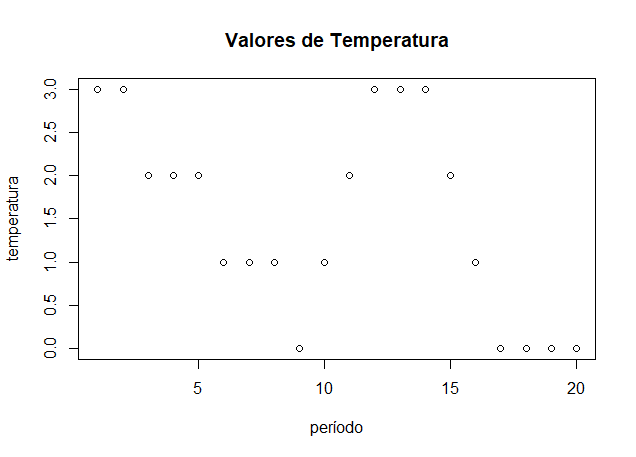
\includegraphics[width=\textwidth]{plotTemp}
 					 \end{subfigure}
 					 \begin{subfigure}[b]{0.6\textwidth}
   						 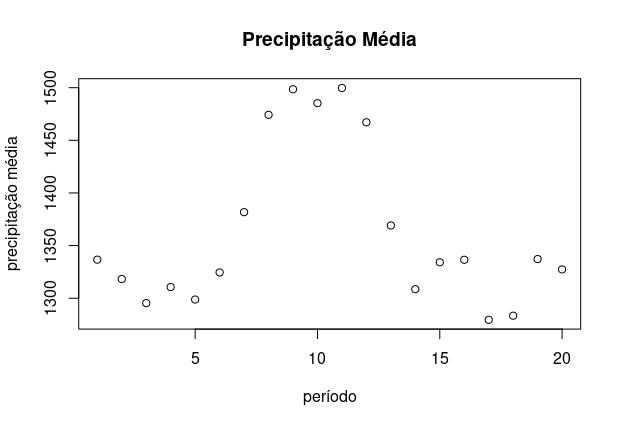
\includegraphics[width=\textwidth]{precMedia}
 					 \end{subfigure}
 				\end{figure}
 				
 				
 				\begin{figure}
 					 \begin{subfigure}[b]{0.6\textwidth}
   						 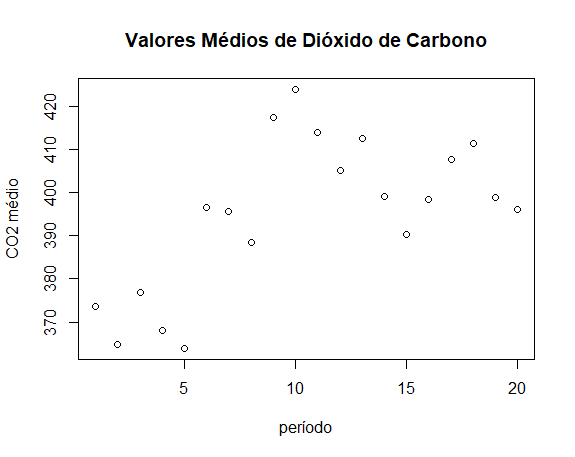
\includegraphics[width=\textwidth]{CO2}
 					 \end{subfigure}
 					 \begin{subfigure}[b]{0.6\textwidth}
   						 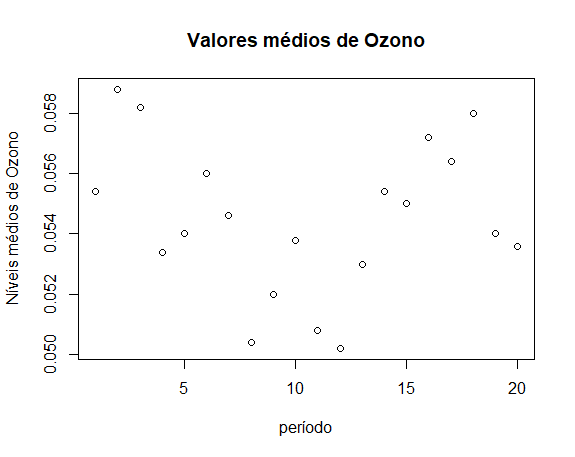
\includegraphics[width=\textwidth]{Ozono}
 					 \end{subfigure}
 				\end{figure}

\newpage

		\subsection*{Alínea 2}
			\paragraph{}
				Descreva o modelo, identificando na família exponencial a distribuição da variável resposta \textit{Y} - Poisson($\lambda$) - e identificando a função ligação entre a média de \textit{Y} e o preditor linear.

			\subsection*{Resolução}
				Uma vez que estamos a ajustar um modelo de regressão Poisson com ligação identidade ao conjunto de dados fornecido, temos que, para a função de ligação entre a média Y e o preditor linear, a seguinte função:
				\begin{equation*}	
				 	g(\mu) = \mu
				\end{equation*}
				Também sabemos que o preditor linear($\eta$) tem a seguinte fórmula:
				\begin{equation*}	
				 	\eta = \beta_{0}z_{i1} +  \beta_{1}z_{i2} + ... +  \beta_{k}z_{i(k+1)} <=> \eta = z'_{i}\beta
				\end{equation*}
				 e que $\mu = \eta$. Pelo que, ficamos com a função de ligação igual a:
				\begin{equation*}	
				 	g(\mu) = \eta
				\end{equation*}


		\subsection*{Alínea 3}
			\paragraph{}
				Escreva a função de log-verosimilhança dos dados e as equações de verosimilhança para estimar os coeficientes de regressão $\beta$ do modelo.

			\subsection*{Resolução}
				A f.m.p da distribuição de Poisson é: 
				\begin{equation*}
					f(y| \lambda)=\frac{ (e^{-\lambda}*\lambda^{y})}{y!}
				\end{equation*}
				A função verosimilhança pode ser calculada da seguinte forma: \paragraph{}
				
				\begin{align*}
					L(\lambda)&= f( (y_{i}, ..., y_{n}) | \lambda) \\					
						  &= \prod_{i=1}^{n} f(y_{i} | \lambda)			
						  = \prod_{i=1}^{n} \frac{ (e^{-\lambda}*\lambda^{y_i})}{y_i!} 				
						  = \prod_{i=1}^{n} \lambda^{y_{i}}*\frac{e^{-\lambda}}{y_{i}!} \\			
						&= e^{-n\lambda}*\frac{\lambda^{\sum_{i=1}^{n} y_{i}}}{\prod_{i=1}^{n} y_{i}!} \\
				\end{align*}		
				
	
				Sabendo que a função log-verosimilhança corresponde a  $ln(L(\lambda))$ temos que:

				\begin{align*}
				ln((L(\lambda)))=ln\left(e^{-n\lambda}*\frac{\lambda^{\sum_{i=1}^{n} y_{i}}} {\prod_{i=1}^{n} y_{i}!}\right)=	\\	
				= ln(e^{-n\lambda})+ln\left(\frac{\lambda^{\sum_{i=1}^{n} y_{i}}} {\prod_{i=1}^{n} y_{i}!}\right)= 		\\		
				= -n\lambda + \left(\sum_{i=1}^{n} y_{i}\right)ln \lambda - ln\left(\prod_{i=1}^{n} y_{i}!\right)\\
				\end{align*}		

				Segundo o enunciado, temos que ajustar um modelo de regressão Poisson com ligação identidade. Como tal, temos que $\mu$ = $\lambda$ = $\eta$ . Também sabemos que $\eta = z'_{i}\beta$, para as duas equações anteriores, temos que:\\ \\
				\begin{equation*}
					L(\beta) = e^{-nz'_{i}\beta}\frac{\left(z'_{i}\beta\right)^{\sum_{i=1}^{n} y_{i}}}{\prod_{i=1}^{n} y_{i}!}\\
				\end{equation*}

				\begin{equation*}
					l(\beta) = ln(L(\beta))= -nz'_{i}\beta + \left(\sum_{i=1}^{n} y_{i}\right)ln \left(z'_{i}\beta\right) - ln\left(\prod_{i=1}^{n} y_{i}!\right)\\
				\end{equation*}

				Por último sabemos que as equações de verosimilhança correspondem à derivada parcial da função log-verosimilhança em função do $\beta_j$, sendo $j$ um dos parâmetros em estudo: 
				\begin{equation*}
					\frac{\partial l(\beta)}{\partial \beta_{j}} = \sum_{i=1}^{n}\frac{\partial l_{i}(\beta)}{\partial \beta_{j}} = 0 \Leftrightarrow \sum_{i=1}^{n}\frac{(y_{i}-\mu_{i})z_{ij}}{Var(Y_{i})}\frac{\partial \mu_{i}}{\partial \eta_{i}} = 0  \quad \quad, j = 1, ..., p
				\end{equation*}

				\subsection*{Alínea 4}
			\paragraph{}
				Obtenha a função score e a matriz de informação de Fisher do modelo.

			\subsection*{Resolução}
				A função score pode ser calculada através da derivação da função log-verosimilhança em função do $\beta$ , ou seja, 
				\begin{equation*}
					S(\beta) = \frac{\partial l(\beta)}{\partial \beta},
				\end{equation*}

		
				Temos que:
				\begin{align*}
					S(\beta) = \frac{\partial l(\beta)}{\partial \beta} 
						     &=\frac { \partial \left( -nz'_{i} \beta + \left(\sum_{i=1}^{n} y_{i}\right)ln(z'_{i} \beta) - ln\left(\prod_{i=1}^{n} y_{i}!\right)\right)}{\partial \beta}\\ 
						     &= -nz'_{i} + \sum_{i=1}^{n}y_{i} \frac {(z'_{i}\beta)'}{z'_{i} \beta} - 0 
                                                                     = -nz'_{i} +\sum_{i=1}^{n} y_{i} \frac {z'_{i}}{z'_{i} \beta}\\
				\end{align*}

				Usando a função score, podemos calcular a matriz hessiana a partir da seguinte forma:
			\begin{align*}
				H(\beta)= l(\beta)'' = S(\beta)' = \left(-nz'_{i} + \sum_{i=1}^{n}y_{i} \frac{1}{\beta}\right)' \\
					 = 0 + \left(\sum_{i=1}^{n}y_{i}\right)' \frac{1}{z_{i}'\beta} +  \sum_{i=1}^{n}y_{i} \left(\frac{1}{\beta} \right)' \\
					= 0 + 0 + \sum_{i=1}^{n}y_{i}\left(\frac{1'*(\beta)-1*(\beta)'}{(\beta)^2}\right) \\
					= \sum_{i=1}^{n}y_{i} \left(\frac{-1}{\beta^2}\right)
			\end{align*}

			A partir da fórmula obtida anteriormente, podemos obter a matriz de Informação de Fisher, fazendo:
			\begin{align*}
				\Im(\beta)=E[-H(\beta)] = E\left[- \sum_{i=1}^{n}y_{i} * \left(\frac{-1}{\beta^2}\right) \right] = E\left[\sum_{i=1}^{n}y_{i} * \left(\frac{1}{\beta^2}\right)\right]
			\end{align*}

			Como não depende de $x_{1}, ...., x_{n}$, temos que 

			\begin{align*}
				\Im(\eta)=E[-H(\eta)] = \sum_{i=1}^{n}y_{i} * \left(\frac{1}{\beta^2}\right)
			\end{align*}

			Outra alternativa ao cálculo da matriz é através do produto matricial, dado por:

			\begin{equation*}
				\Im(\eta)=\textbf{Z'WZ}, \quad W = diag \left(w_i* = \frac{\left(\frac{\partial \mu_i}{\partial \eta_i}\right)^2}{Var (Y_i)}\right)
			\end{equation*}

			Sendo $Z$ a matriz das covariáveis onde a primeira coluna são $1$'s e as restantes os valores das covariáveis $x_1$, $x_2$ e $x_3$.
			
			\begin{align*}
				\begin{bmatrix} 
					1 & z_{11} & z_{12} & ... & z_{1p}\\
					1 & z_{21} & z_{22} & ... & z_{2p}\\
					: & : & : & & :\\
					1 & z_{n1} & z_{n2} & ... & z_{np}\\
				\end{bmatrix}
			\end{align*}

\newpage

		\subsection*{Alínea 5}
			\paragraph{}
				Construa e programe no \textbf{R} o algoritmo iterativo de estimação dos coeficientes de regressão que se baseia no método dos scores de Fisher. Estime os coeficientes do seu modelo, apresente-os e comente. Apresente em gráfico igualmente os resíduos do modelo e comente.

			\subsection*{Resolução}
				
			Neste momento, podemos escrever a recursão que nos dará os valores de $\beta$ através estimação dos coeficientes de regressão que se baseia no método dos scores de Fisher. Utilizando a expressão podemos obter o próximo $\beta$ e assim sucessivamente até chegarmos ao melhor valor.
			
				\begin{equation*}
					\beta^{k+1} = \left(\textbf{Z'W}^{(k)}\textbf{Z}\right)^{-1}  \textbf{Z'W}^{(k)}\textbf{u}^{(k)}
				\end{equation*}
			
			Sendo $k$ o número da iteração currente, $u^{(k)}$ um vetor de elementos genéricos dado por:
			
				\begin{align*}
					u_i^{(k)} &= \sum_{j=1}^{p}z_{ij}\beta_j^{k} + (y_i - \mu_i^{(k)})\frac{\partial \eta_i^{(k)}}{\partial \mu_i^{(k)}}
					= \eta_i^{(k)} + (y_i - \mu_i^{(k)})\frac{\partial \eta_i^{(k)}}{\partial \mu_i^{(k)}}\\
					&= \eta_i^{(k)} + (y_i - \eta_i^{(k)})\frac{\partial \eta_i^{(k)}}{\partial \eta_i^{(k)}}
					= \eta_i^{(k)} + y_i - \eta_i^{(k)}
					= y_i
				\end{align*}
			
				\begin{figure}[!h]
 					 \begin{subfigure}[b]{0.62\textwidth}
   						 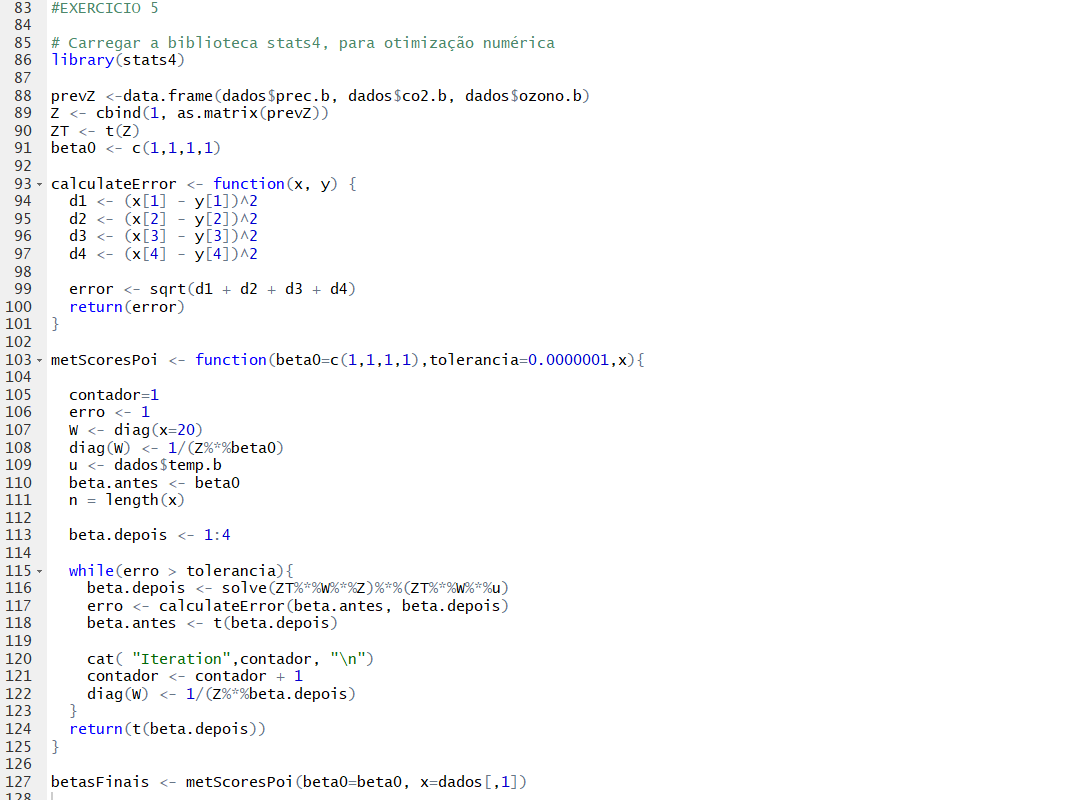
\includegraphics[width=\textwidth]{ex5)1}
 					 \end{subfigure}
 					 \begin{subfigure}[b]{0.75\textwidth}
   						 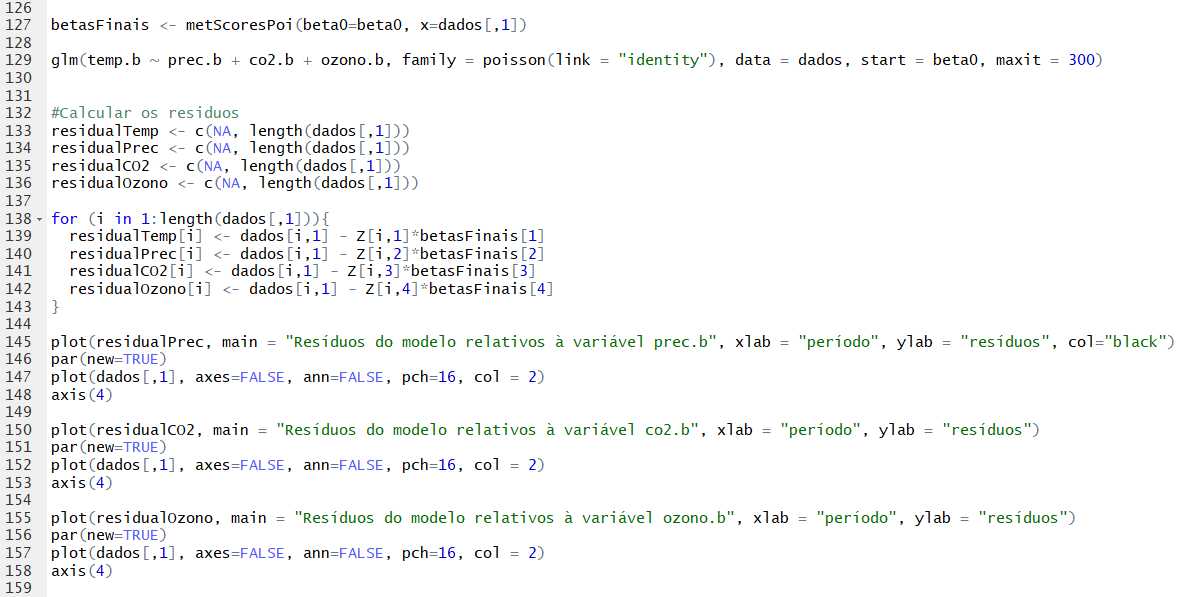
\includegraphics[width=\textwidth]{ex5)2}
 					 \end{subfigure}
 				\end{figure}
			
\newpage			
			
			\subsection*{Análise}
			
			A fórmula usada para o calculo dos resíduos foi:
			
			\begin{equation*}
				\hat{\epsilon} = Y - \hat{Y} = Y - X\hat{\beta}
			\end{equation*}
			
			\noindent Que nos permitiu obter os seguintes gráficos, que compara os residuos de cada covariável com a variável de resposta.
			
				\begin{figure}[!h]
 					 \begin{subfigure}[b]{0.6\textwidth}
   						 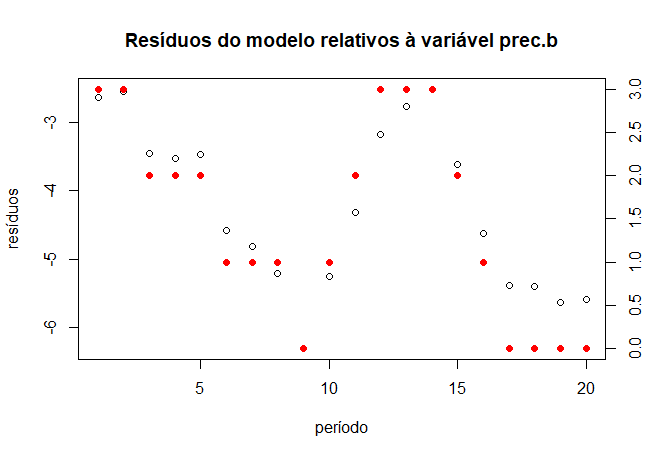
\includegraphics[width=\textwidth]{residuosPrec}
 					 \end{subfigure}
 					 \begin{subfigure}[b]{0.6\textwidth}
   						 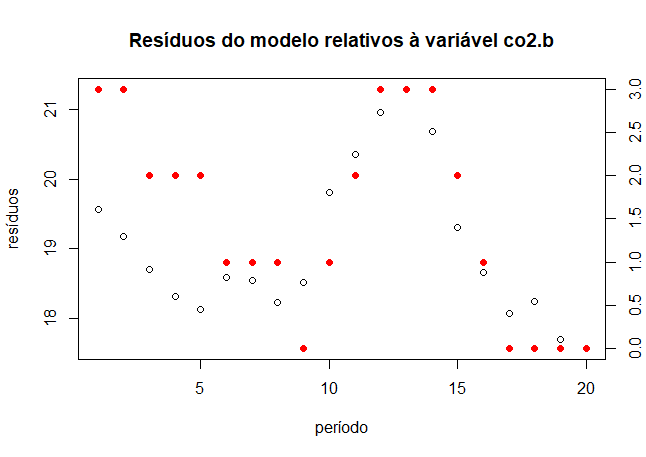
\includegraphics[width=\textwidth]{residuosCO2}
 					 \end{subfigure}
 					 \begin{subfigure}[b]{0.6\textwidth}
   						 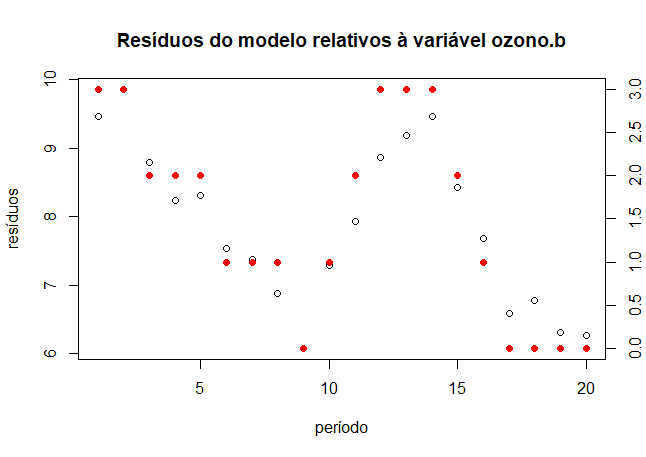
\includegraphics[width=\textwidth]{residuosOzono}
 					 \end{subfigure}
 				\end{figure}
 				
 				Observando os gráficos obtidos, podemos concluir que, comparando a variável de resposta Y (temperatura) com o cálculo dos resíduos para as restantes variáveis, a variável dióxido de carbono é a que, em termos médios se afasta mais dos valores de Y. Por outro lado, as variáveis ozono e precipitação, parecem ser semelhantes nesta comparação. No entanto, consideramos que a primeira destas duas se encontra mais próxima da variável de resposta e, por isso, podemos concluir que o ozono é a variável que mais afeta as baixas temperaturas num dado local.			
			
\end{document}